\documentclass[12pt,oneside,a4paper]{article}

\pdfminorversion 4

\usepackage[margin=1in]{geometry}
\usepackage[toc,page]{appendix}
\usepackage{amsmath,amsfonts,amssymb}
\usepackage{graphicx, wrapfig}
\usepackage{color}
\usepackage{float}
\usepackage{tabularx,colortbl}

\usepackage{amsthm}

\usepackage[font=footnotesize]{caption}
\usepackage{subcaption}

\usepackage{fancyhdr}
\pagestyle{fancy}
\lhead{PHY 905 Project 2}
\rhead{Nicholas Miller}

\newcommand{\br}{\vec {\bf r}}
\newcommand{\bv}{\vec {\bf v}}
\newcommand{\ba}{\vec {\bf a}}
\newcommand{\bF}{\vec {\bf F}}

\newcommand{\dt}{\Delta t}

% -------------------------------------------------

\renewcommand{\arraystretch}{1.25} 
\renewcommand{\baselinestretch}{1.0}

\begin{document}

\section{Theory}

\subsection{Interacting Argon Atoms}

The goal of this project is to simulate the dynamics of a system of $N$ argon atoms.  Interactions between atoms are approximated by the Lennard-Jones potential energy function:
\begin{equation}
\label{eq:LJ_PTE}
V\left(\br_i, \br_j\right) = 4\varepsilon \left[\left(\frac{\sigma}{R}\right)^{12} - \left(\frac{\sigma}{R}\right)^{6}\right]
\end{equation}
where $R = |\br_i-\br_j|$ is the distance between the centers of atom $i$ and atom $j$.  The constants $\varepsilon$ and $\sigma$, along with the mass $m$, are set to unity for this project.  The force on atom $i$ due to all other atoms in the system is:
\begin{equation}
\bF(\br_i(t)) = \sum\limits_{j\neq i} 24\left[2\left(\frac{1}{R}\right)^{14} - \left(\frac{1}{R}\right)^{8}\right]\left(\br_i(t)-\br_j(t)\right)
\end{equation}
An equation of motion is now written using Newton's classical laws for the $i^\text{th}$ atom:
\begin{equation}
\label{eq:ODE}
\frac{d^2 \br_i(t)}{dt^2} = \frac{\bF(\br_i(t))}{m} = \bF(\br_i(t))
\end{equation}
Given proper initial conditions, these $3N$ ordinary differential equations are integrated in time to simulate the argon atoms dynamics.

\subsection{Velocity Verlet Algorithm}

Eqn. (\ref{eq:ODE}) is integrated in time using the well known Velocity Verlet Algorithm, which is derived from Taylor expansions.  This algorithm updates both particle position and velocities in a three step process:
\begin{enumerate}
	\item Define $\ba_i(t) = \bF(\br_i(t))$
	\item $\br_i(t+\dt) = \br_i(t) + \bv_i(t)\dt + \frac{1}{2}\ba_i(t)\dt^2$
	\item $\ba_i(t+\dt) = \bF(\br_i(t+\dt))$
	\item $\bv_i(t+\dt) = \bv_i(t) + \frac{1}{2}\left[\ba_i(t+\dt)+\ba_i(t)\right]$
\end{enumerate}
Here, $\dt$ is the time step size of the time integration.  The Velocity Verlet algorithm requires initial conditions for both particle positions and velocities, and will compute updated positions, velocities, and accelerations at each time step.

\subsection{Initial Conditions}

Initial conditions must be properly prescribed in order to integrate the equations of motion.  For the positions,  the argon particles are initially placed on a face centered cubic (FCC) lattice, shown in Figure \ref{fig:fcc}.
\begin{figure}[!h]
	\centering
	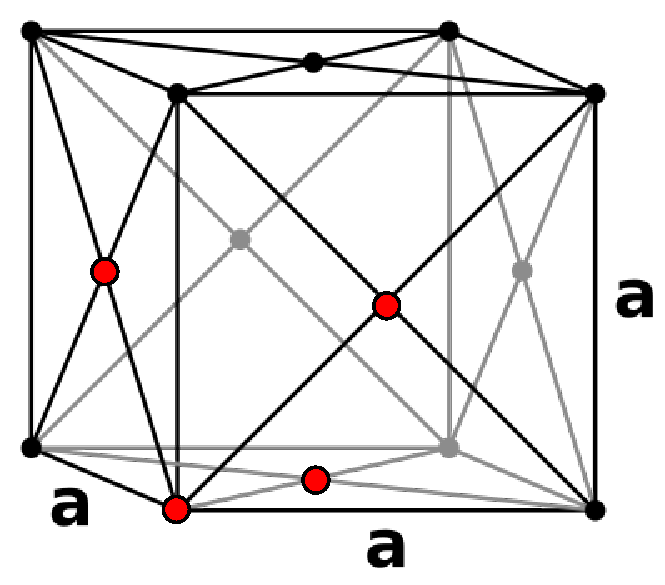
\includegraphics[width=0.5\textwidth]{./fcc.pdf}
	\caption{The face centered cubic (FCC) initial particle positions for the Velocity Verlet algorithm.}
	\label{fig:fcc}
\end{figure} 
A subset of the FCC lattice positions, shown in red, can then be used as a template and iterated in all spatial directions until the desired amount of atoms are present in the system.

Next, the initial velocities must be set.  A good initial velocity is generated from a Gaussian probability distribution:
\begin{equation}
P(x) = \frac{\exp\left[-\left(x-x_0\right)^2/\left(2\sigma\right)^2\right]}{\sqrt{2\pi \sigma^2}}
\end{equation}
For this code, the center and variance were set to $x_0=0$ and $\sigma^2=1$, respectively.  Since the random initial velocities are distributed around zero, the total momentum will not be exactly zero.  To prevent the system drifting in space, the random initial velocities are transformed to a center of mass reference frame:
\begin{equation}
\bv_0 \rightarrow \bv_0 - \frac{1}{N}\sum\limits_{i=1}^N \bv_i
\end{equation}
The final part of initializing the velocities is to then scale them in order to get the desired temperature:
\begin{equation}
\bv_0 \rightarrow \sqrt{\frac{3(N-1)T_\text{desired}}{\sum\limits_{i=1}^N \bv_i}}\bv_0 
\end{equation}

\subsection{Periodic Boundary Conditions}

Now that the integration method and initial conditions are set, boundary conditions on the system of argon atoms are the final piece of the puzzle in order to simulate the dynamics.  Periodic boundary conditions (PCB) were chosen here, but a hard ``box-like'' boundary condition could also be imposed.  
\begin{figure}[!h]
	\centering
	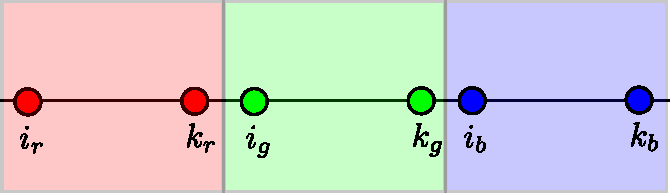
\includegraphics[width=0.75\textwidth]{./minimum-image-convention.pdf}
	\caption{The minimum image convention illustration in one dimension.}
	\label{fig:mic}
\end{figure} 
The PCBs are needed in two aspects of the Velocity Verlet algorithm.  The first is computing the accelerations between particles, and the second is when a particle leaves the computational domain created by the initial FCC lattice positions.

The \emph{minimum image convention} is used to compute the accelerations between particles in the periodic FCC lattice.  An illustration of the method is shown in Figure \ref{fig:mic}.  If $R_{i_g k_r} = |\br_{i_g} - \br_{k_r}|$ is less than $R_{i_r k_r} = |\br_{i_r} - \br_{k_r}|$, then the stronger force with distance  $R_{i_g k_r}$ is used for computing the acceleration and the weaker force with distance $R_{i_r k_r}$ is neglected.  Since the lattice is periodic, then the minimum image convention can be written in the succinct algorithm:
\begin{itemize}
	\item If $R_{i k} = |\br_{i} - \br_{k}| > \frac{L}{2}$
	\begin{itemize}
		\item If $R_{i k} > 0 \rightarrow R_{i k} = R_{i k} + L$
		\item If $R_{i k} < 0 \rightarrow R_{i k} = R_{i k} - L$
	\end{itemize}
\end{itemize}
This can be visually seen  using Figure \ref{fig:mic}.  When the two particles in the red unit cell are separated by a distance larger than half the unit cell size, then the second particle is translated by the unit cell dimension to compute the distance between the red particle and the green particle. 

Using the PCBs for particles which leave the computational domain is much more straight forward.  If the updated particle position is outside of the computational domain, then its position is merely shifted by the size of the computational domain $\br_i \rightarrow \br_i + L$.

\subsection{Andersen Thermostat}

An Andersen Thermostat was implemented to fix the temperature at a desired constant.  This thermostat assumes that part of the system has an instantaneous interaction with fictional particles which exchange energy with the argon particles.  Energy exchange between the thermostat and the Argon particles is implemented by replacing the particle momentum of some particles with a new momentum drawn from a Gaussian distribution.  The Andersen Thermostat algorithm is:
\begin{itemize}
	\item For velocity $\bv_i$, if $\left(\right.$\emph{Uniform random number} $\left.\in \left[0, 1\right] \right) \leq 1-\exp\left(\nu \dt\right)$
	\begin{itemize}
		\item $\bv_i \rightarrow \sqrt{\frac{k_B T}{2 m}} \text{Gauss}\left(0, 1\right)$
	\end{itemize}
\end{itemize}
Here, $\text{Gauss}\left(0, 1\right)$ is a Gaussian random number between $0$ and $1$.

\section{Results}

\subsection{Temperature and Energy Measurements}

For this report, four numerical measurements are taken in order to prove the validity of the code.  These are:  instantaneous temperature, kinetic energy, potential energy, and total energy.  The temperature at each time step $T_n$ is computed using the equipartition formula:
\begin{equation}
3(N-1)k_B T = \frac{m}{2}\sum\limits_{i=1}^{N}|\bv_i|^2
\end{equation}
Total energy is computed as the sum of the kinetic and potential energy:
\begin{equation}
E = KE + PE = \frac{m}{2}\sum\limits_{i=1}^{N}|\bv_i|^2 + \sum\limits_{i=1}^{N}\sum\limits_{j=1}^{N} V\left(\br_i, \br_j\right)
\end{equation}
where $V\left(\br_i, \br_j\right)$ is given by Eqn. (\ref{eq:LJ_PTE}).

\subsection{$N = 256$, $T = 5$}

The temperature for an $N=256$ particle system with a desired temperature of $T = 5 K$ is shown in Figure \ref{fig:temp}.  A total of $20,000$ time steps were used in this simulation with $\dt = 10^{-4}$, and the thermostat with $\nu=1$, $10$, and $100$ was turned off after $10,000$ time steps.
\begin{figure}[!h]
	\centering
	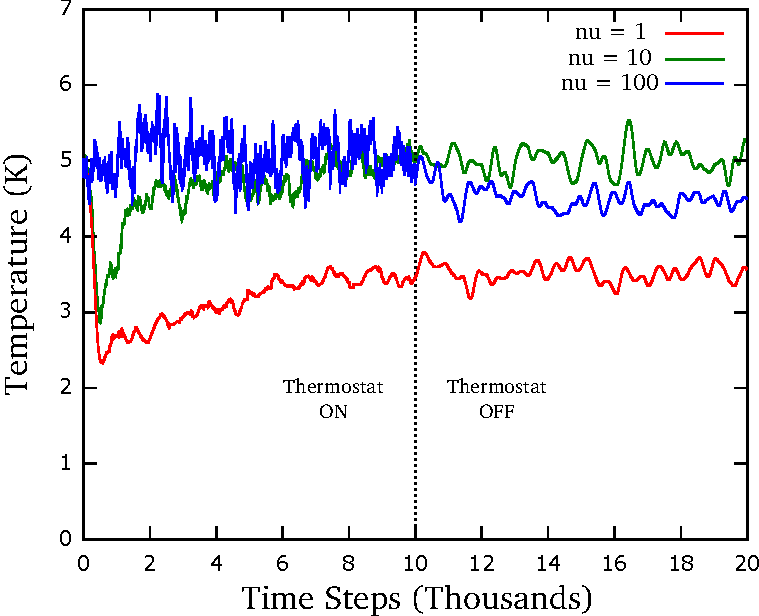
\includegraphics[width=0.7\textwidth]{../cpp/results/Temperature.pdf}
	\caption{Molecular dynamics temperature result for $N=256$ particles at $T = 5 K$ after $20,000$ time steps.}
	\label{fig:temp}
\end{figure} 
This result proves the validity of the molecular dynamics code and at the same time provides some interesting results.  The first noticeable characteristic of the temperature is that it tries to drift away from the desired value for $\nu=1$ and $10$, but the thermostat is able to slowly bring it back.  The temperature with $\nu=100$ suffers from much more wild oscillations than the others, however, and starts to drift away from the desired temperature after the thermostat is turned off.  

Since the thermostat with $\nu=10$ performs the best over this time range, this parameter will be used to calculate the energy of the system.  Figure \ref{fig:energy} shows the calculated kinetic, potential, and total energy with the same parameters and $\nu=10$.  
\begin{figure}[!h]
	\centering
	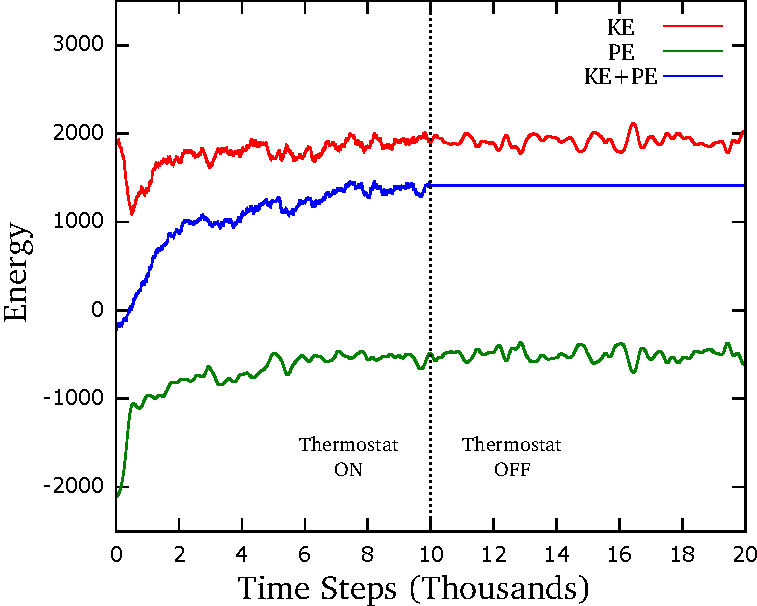
\includegraphics[width=0.7\textwidth]{../cpp/results/Energy.pdf}
	\caption{Molecular dynamics energy result for $N=256$ particles at $T = 5 K$ after $20,000$ time steps.  Here, KE stands for kinetic energy and PE stands for potential energy.}
	\label{fig:energy}
\end{figure} 
After the thermostat is turned off, the total energy is constant.  This matches intuition as after the thermostat is turned off, no energy is entering of leaving the system.  This energy result also provides an excellent validation that the code is in fact valid and performing as expected.

\end{document}
